%%%%%%%%%%%%%%%%%%%%%%%%%%%%%%%%%%%%%%%%%%%%%%%%%%%%%%%%%%%%%%%%%%%%%%%%%%
% Fundamental Current i^1_1a for M3C with RL-Load
%%%%%%%%%%%%%%%%%%%%%%%%%%%%%%%%%%%%%%%%%%%%%%%%%%%%%%%%%%%%%%%%%%%%%%%%%%
\begin{solutionfigure}[htb]

    %   \documentclass{standalone}
    %   \usepackage{pgfplots}
    %   \pgfplotsset{compat=1.18} % Kompatibilität für neuere Versionen
           \centering
           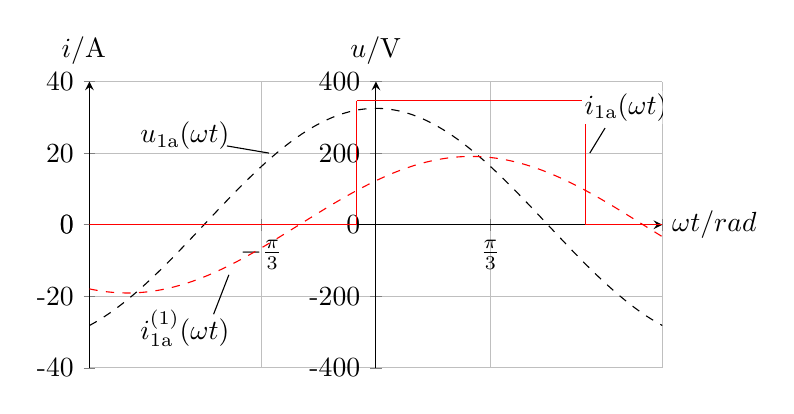
\begin{tikzpicture}
                \pgfplotsset{set layers}
               \begin{axis}[
                    % x/y range adjustment
                    scale only axis,
                    xmin=-150, xmax=150,
                    ymin=-40, ymax=40,
                    samples=500,
                    axis y line=center,
                    axis x line=middle,
                    extra y ticks=0,
                    % Label text
                    xlabel={$\omega t / \text{rad}$},
                    ylabel={$u/\mathrm{V}$},
                    % Label adjustment
                    x label style={at={(axis description cs:1,0.5)},anchor=west},
                    y label style={at={(axis description cs:0.5,.97)},anchor=south,yshift=0.2cm},
                    width=0.6\textwidth,
                    height=0.3\textwidth,
                    % x-Ticks
                    xtick={-150,-60,0,60,150},
                    xticklabels={,$-\frac{\pi}{3}$,0,$\frac{\pi}{3}$,,},
                    xticklabel style = {anchor=north},
                    % y-Ticks
                    ytick={40,20,0,-20,-40},
                    yticklabels={400,200,0,-200,-400},
                    yticklabel style = {anchor=east},
                    % Grid layout
                    grid,
                    %grid style={line width=.1pt, draw=gray!10},
                    %major grid style={line width=.2pt,draw=gray!90},
                ]
               % Voltage u1a(wt)
               \addplot[black, domain= -150:150,dashed] {32.5*cos(x)};
        
            % Label of u1a           
            \node[black, fill=white, inner sep = 1pt, anchor = south] at (axis cs:-100,20) {$u_{\mathrm{1a}}(\omega t)$};
            
            % Line for u1a
            \draw[thin, black] (-78,22) -- (-56,20);
           \end{axis}
           \begin{axis}[
            % x/y range adjustment
            scale only axis,
            ymin=-40, ymax=40,
            xmin=-150, xmax=150,
            axis x line=none, 
            samples=500,
            axis y line=left,
            axis x line=middle,
            extra y ticks=0,
            % Label text
            ylabel={$i/\mathrm{A}$},
            % Label adjustment
            y label style={rotate = -90,at={(axis description cs:-0.01,.97)},anchor=south,yshift=0.2cm},
            width=0.6\textwidth,
            height=0.3\textwidth,
            % y-Ticks
            ytick={40,20,0,-20,-40},
            yticklabels={40,20,0,-20,-40},
            yticklabel style = {anchor=east},
            % Grid layout
            grid,
            %grid style={line width=.1pt, draw=gray!10},
            %major grid style={line width=.2pt,draw=gray!90},
        ] 
        % Current i^1_1a(wt) fundamental
        \addplot[red, domain= -150:150, dashed] {19.07*cos(x-(49.9))};
        % Current i1a(wt)
        \addplot[color=red,solid] coordinates{
            (-150,0)
            (-10.09, 0)
        };                 
           \addplot[color=red,solid] coordinates{
            (-10.09,0)
            (-10.09, 34.6)
        };                   
           \addplot[color=red,solid] coordinates{
               (-10.09,34.6)
               (109.9, 34.6)
           };  
           \addplot[color=red,solid] coordinates{
            (109.9,0)
            (109.9, 34.6)
        };
        \addplot[color=red,solid] coordinates{
            (109.9,0)
            (150, 0)
        };    
           % Label of i1a
           \node[black, fill=white, inner sep = 1pt, anchor = south] at (axis cs:131,28) {$i_{\mathrm{1a}}(\omega t)$};
           % Label of i^1_1a fundamental 
           \node[black, fill=white, inner sep = 1pt, anchor = south] at (axis cs:-100,-35) {$i^\mathrm{(1)}_{\mathrm{1a}}(\omega t)$}; 
            % Line to i1a
            \draw[thin, black] (112,20) -- (120,27);
            % Line to i^1_1a fundamental
            \draw[thin, black] (-85,-25) -- (-77,-14);
           \end{axis}         
           \end{tikzpicture}
           \caption{Fundamental current component $i^\mathrm{(1)}_{\mathrm{1a}}(\omega t)$ for $\alpha = 0.871$.}
           \label{sfig:ex06_current_signals_6_1_4b}
   \end{solutionfigure}